\chapter{Work description}
\label{cap:descripcionTrabajo}

We designed a simple structure to organize all the scripts. As we are implementing different versions of the engine, there are specific modules that are compulsory to have well distinguished and possibly selected between them. Those modules are presented in the following Section~\ref{sec:modules}.

\vspace{1em}

\noindent Next, the key point is how to represent each required structure, including the board, chess pieces, precomputed tables, transposition tables, etc., as discussed in Section~\ref{sec:code}.

\section{Modules}
\label{sec:modules}

Each module is responsible for a specific aspect of the chess engine's functionality. The good part about this modular design is that it ensures clarity, maintainability, and the ability to test and improve individual components independently even more so when it comes to development with more people.

\subsection{Board}

\noindent This module handles the representation of the chessboard, as previously mentioned in Section~\ref{sec:board}, and the state of the game. It includes:
\begin{itemize}
    \item Representation of the chessboard with its pieces using bitboards for efficiency.
    \item Functions to make and unmake moves, including special moves like castling and en passant.
    \item Updating game state variables, such as castling rights or the half-move counter.
\end{itemize}

\noindent This module is vital, as it provides the data structures and operations required by other modules.

\subsection{Move generator}

\ldots

\subsection{Move ordering}

\ldots

\subsection{Evaluation}

\ldots

\subsection{Search}

\ldots

\subsection{UCI}

\ldots

\section{Code implementation}
\label{sec:code}

All the code implementation is written in C++. However, the algorithms will be represented in pseudocode since the focus is on their logic rather than their specific implementation. The data structures, on the other hand, will be described using the programming language employed.

\subsection{Data representation}

\subsubsection{Square}

There are 64 possible squares on a chessboard so the first thought is to use a 6-bit structure which seem like a perfect match ($2^6 = 64$). However, modern processors are optimized to work with data sizes aligned to multiples of 8 bits (1 byte). Then, using 6 bits would require packing the data into more complex structures, which could introduce additional overhead in terms of bit manipulation and memory access. We preferred clarity and performance over micro-optimizations that complicate readability so we used a \texttt{uint8\_t} to describe a square.

\vspace{1em}

\noindent Moreover, masks are extremely useful for efficiently identifying and manipulating the squares on a chessboard using bitwise operations. Some of these masks are defined as constants in the code and others are calculated during compilation time. For example, they can be used to identify the column of a square or simply placing a new piece on board.

\begin{lstlisting}
    class Square {
        uint8_t sq_value;

        constexpr bool is_valid() const {
            return sq_value < 64U;
        }

        constexpr uint64_t mask() const {
            return is_valid() ? 1ULL << sq_value : 0ULL;
        }

        // Calculating the column of a square (sq_value % 8)
        constexpr int col() const {
            return is_valid() ? sq_value & 7U : COL_INVALID;
        }
    }

    // Placing a piece by setting the bit corresponding to the
    // square to 1
    const uint64_t mask = square.mask();
    bitboard_all |= mask;
\end{lstlisting}

\noindent Just to clarify, \texttt{sq\_value} must be a value between $0$ and $63$, inclusive, for the 64 squares on a chessboard. To calculate the column of a square, an AND operation is applied: \texttt{sq\_value \& 7U} extracts the 3 least significant bits, which correspond to the column of the square. Columns are enumerated from $0$ (A) to $7$ (H).

\subsubsection{Piece and PieceType}

They are simply enumerations where each piece and piece type correspond to an integer number to improve code readability.

\begin{lstlisting}
    enum class Piece : int
    {
        W_PAWN = 0,
        W_KNIGHT = 1,
        W_BISHOP = 2,
        ...
        B_QUEEN = 10,
        B_KING = 11,
        EMPTY = 12,
        NUM_PIECES = 13
    };

    enum class PieceType : int
    {
        PAWN = 0,
        KNIGHT = 1,
        BISHOP = 2,
        ROOK = 3,
        QUEEN = 4,
        KING = 5,
        EMPTY = 6,
        NUM_PIECES = 7
    };
\end{lstlisting}

\subsubsection{Move and MoveType}

There are four types of moves: normal, promotion, en passant, and castling. These are represented using an integer-based enumeration:

\begin{lstlisting}
    enum class MoveType
    {
        NORMAL = 0,
        PROMOTION = 1,
        EN_PASSANT = 2,
        CASTLING = 3
    };
\end{lstlisting}

\noindent Meanwhile, moves are represented as a combination of two squares (the origin square and the destination square), 2 bits for the promotion piece, and 2 bits for the move type, all encoded in a \texttt{uint16\_t}. In this case, each square is represented using 6 bits, resulting in a total of 16 bits $(6 + 6 + 2 + 2 = 16~\mathrm{bits})$. Each bit field has a unique mask and its specific shift, which must remain unchanged throughout the development.

\subsubsection{Game State}

The game state must store important information during the game, including the Zobrist hash key of the current position, the number of moves, the en passant square, the castling rights for each side and color, the side to move, the last captured piece, the fifty-move rule counter, the number of pieces, and a flag indicating whether the attacks are updated.

\vspace{1em}

\noindent There are two \texttt{uint64\_t} variables: one for the Zobrist hash key and the other for the remaining bit fields:

\begin{lstlisting}
    class GameState {
        uint64_t zobrist_key;

        // 50 : attacks_updated : 1 if updated, 0 if not
        // 43-49 : num_pieces : 0 to 64 pieces
        // 35-42 : fifty_move_rule_counter : if counter gets to 
        // 100 then game is a draw.
        // 32-34 : last_captured_piece : PieceType::Empty if last
        // move was not a capture.
        // 31 : side_to_move : 0 if white, 1 if black.
        // 30 : castle_king_white : 1 if available, 0 if not.
        // 29 : castle_queen_white : 1 if available, 0 if not.
        // 28 : castle_king_black : 1 if available, 0 if not.
        // 27 : castle_queen_black : 1 if available, 0 if not.
        // 26-20 : en_passant_square : 0-63 if available, >=64 if
        // not available
        // 19-0 : move_number : 0-1048575 number of moves in the 
        // game.
        uint64_t state_register;
    }
\end{lstlisting}

\subsubsection{Board}

For the chessboard, as previously mentioned, bitboards are represented as 64-bit structures using \texttt{uint64\_t}. Since the sign is not relevant, an unsigned type is used.

\vspace{1em}

\noindent The bitboard representation follows the Little-Endian Rank-File Mapping convention also called as LERF. In this mapping, each bit in the 64-bit integer corresponds to a square on the chessboard where the least significant bit (0) is square \texttt{A1}, and the most significant bit (63) is square \texttt{H8}.

\begin{figure}[H]
    \centering
    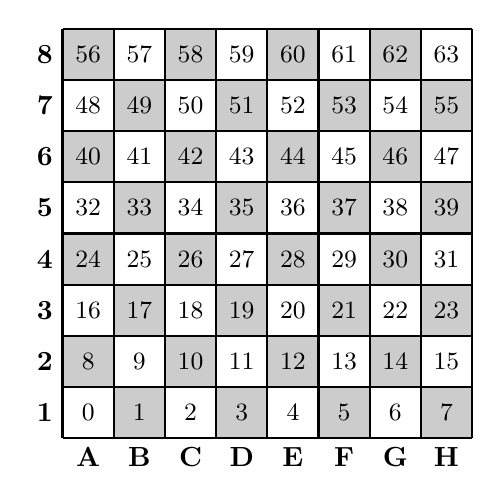
\begin{tikzpicture}[scale=0.65]
        % Draw the chessboard
        \foreach \x in {0,1,...,7} {
            \foreach \y in {0,1,...,7} {
                \pgfmathparse{mod(\x+\y,2) ? "black!20" : "white"}
                \edef\col{\pgfmathresult}
                \fill[\col] (\x,\y) rectangle (\x+1,\y+1);
                
                % Calculate the square index
                \pgfmathtruncatemacro{\num}{\x + 8*\y}
                % Add the number to the square
                \node at (\x+0.5,\y+0.5) {\small \num};
            }
        }

        % Add column labels (A-H)
        \foreach \x [count=\i from 0] in {A, B, C, D, E, F, G, H} {
            % \node[above] at (\i+0.5, 8) {\textbf{\x}}; % Top labels
            \node[below] at (\i+0.5, 0) {\textbf{\x}}; % Bottom labels
        }

        % Add row labels (1-8)
        \foreach \y [count=\i from 0] in {1, 2, 3, 4, 5, 6, 7, 8} {
            \node[left] at (0, \i+0.5) {\textbf{\y}}; % Left labels
            % \node[right] at (8, \i+0.5) {\textbf{\y}}; % Right labels
        }

        % Draw the grid
        \draw[thick] (0,0) grid (8,8);
    \end{tikzpicture}
    \caption{Little-Endian Rank-File Mapping with Coordinates.}
    \label{fig:lerf}
\end{figure}

\noindent \parbox{\textwidth}{There are bitboards for all pieces (\texttt{bitboard\_all}), for each piece color (\texttt{bitboard\_color[0]} and \texttt{bitboard\_color[1]}), and for each piece type (\texttt{bitboard\_piece[Piece]} like \texttt{bitboard\_piece[Piece::W\_QUEEN]})}.

\vspace{1em}

\noindent To identify ray directions on the board, we used the compass rose:

\begin{center}
    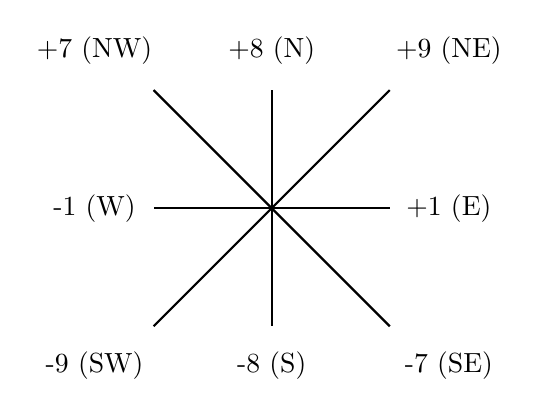
\begin{tikzpicture}
        \node at (0, 2) {+8 (N)};
        \node at (2.25, 2) {+9 (NE)};
        \node at (-2.25, 2) {+7 (NW)};
        \node at (2.25, 0) {+1 (E)};
        \node at (-2.25, 0) {-1 (W)};
        \node at (0, -2) {-8 (S)};
        \node at (2.25, -2) {-7 (SE)};
        \node at (-2.25, -2) {-9 (SW)};
        \draw[thick] (0, 0) -- (0, 1.5);
        \draw[thick] (0, 0) -- (1.5, 1.5);
        \draw[thick] (0, 0) -- (-1.5, 1.5);
        \draw[thick] (0, 0) -- (1.5, 0);
        \draw[thick] (0, 0) -- (-1.5, 0);
        \draw[thick] (0, 0) -- (0, -1.5);
        \draw[thick] (0, 0) -- (1.5, -1.5);
        \draw[thick] (0, 0) -- (-1.5, -1.5);
    \end{tikzpicture}
\end{center}

\noindent This means that, to get the numerical value that identifies the square to the north-east of a given square, you only need to add 9. For example, given the square $f6$ (45), the north-east square $g7$ has a value of 54 (45 + 9 = 54). It is really effective for sliding pieces to calculate their attacks.

\subsubsection{Transposition table}

The transposition table contains a list of entries. These entries are defined as a storage of information about a specific chess position, including its Zobrist key, evaluation score, best move, node type, and search depth.

\ldots

\subsubsection{History}

\ldots

\subsubsection{Move generator information}

\ldots

\subsection{Precomputed data}

Some tables are memory initialized instead of computed, explain it.

\ldots

\section{Additional tools and work}

\ldots

\subsection{Board visualizer using Python}

\ldots

\subsection{Profiling}

Continue in next Chapter~\ref{cap:profiling}.

\ldots

\subsection{Testing engine strength}

Testing and analysis in Chapter~\ref{cap:testing}.

\ldots